\item \points{1a} \textbf{Implementing Goal Conditioned Reinforcement Learning}

We start this problem with a goal-conditioned implementation of
DQN. The $Q$-function takes in the concatenated state and goal as input. You can think of the goal-conditioned implementation as an extended Markov decision process (MDP), where your state space contains both the original state and the goal. We will use this goal-conditioned $Q$-network to
collect episodic data in \texttt{run\_episode.py}.

For this part of the assignment, complete \texttt{run\_episode.py} and run the following command:
\begin{lstlisting}[language=bash]
    python -m goal_conditioned_rl.main --env bit_flip --num_bits=6 --num_epochs=250 --her_type no_hindsight
\end{lstlisting}

The evaluation metrics should be available in tensorboard events logged in \texttt{logs/} by default. \textbf{Verify} the \texttt{eval\_metrics}, that is \texttt{total\_reward} should be above $-40.0$ and success rate
should be $1.0$. This plot illustrates the performance without using HER.

\begin{center}
    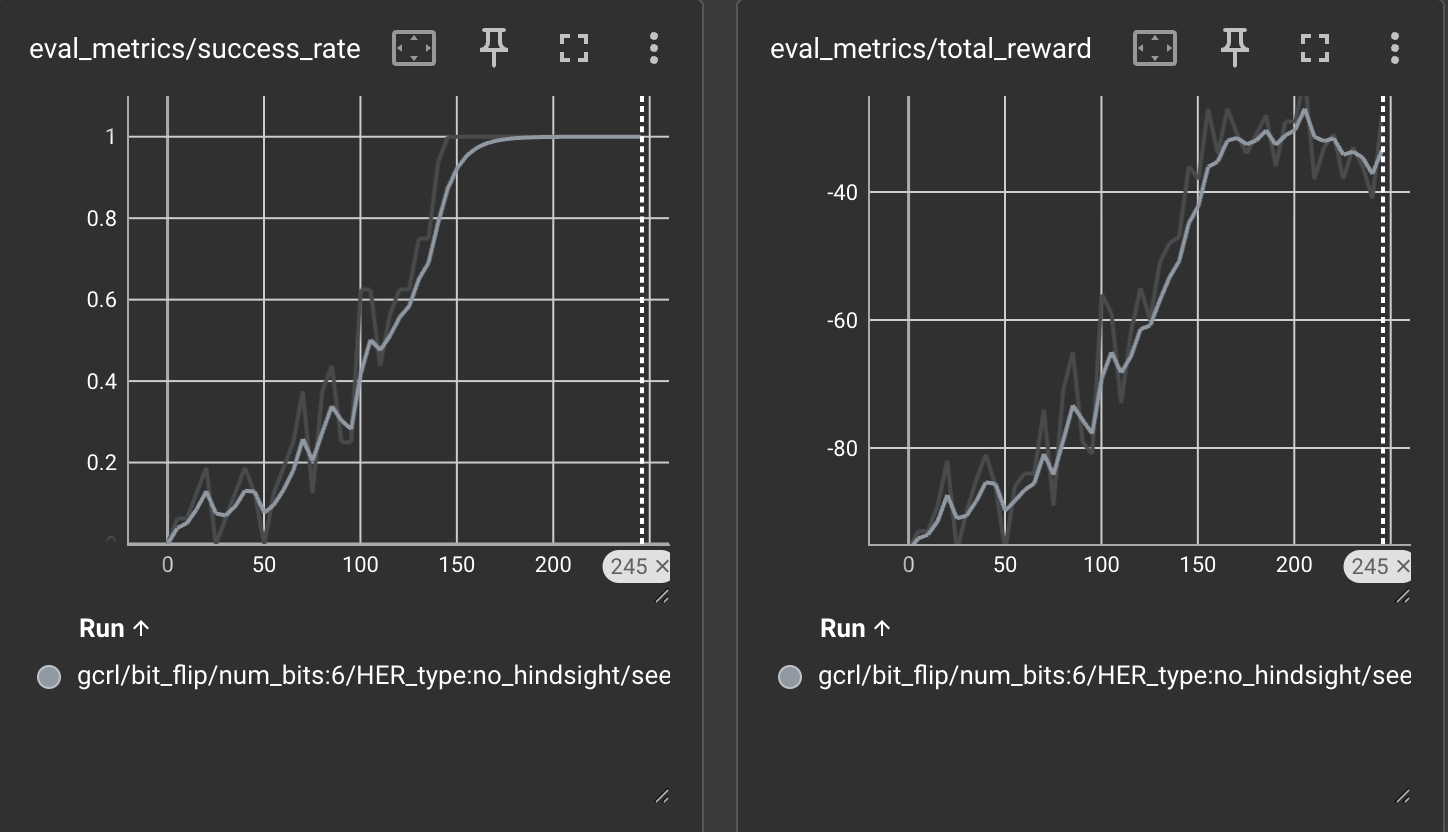
\includegraphics[width=0.5\textwidth]{figures/1a-expect}
\end{center}

\begin{enumerate}[label=(\roman*)]
    \item  For simplicity, we will only consider the \textit{greedy} action with respect to $Q$-network.
Pass this action to \texttt{env.step}.
\item The \texttt{env.step} function returns \texttt{next\_state}, \texttt{reward}, \texttt{done}, \texttt{info}, where \texttt{info} is a
dictionary containing the a boolean under the key '\texttt{successful\_this\_state}', indicating whether the state was successful or not. Use this value to update succeeded,
such that \texttt{run\_episode} returns \texttt{True} if the \textit{policy was successful at any step of the episode}.
To understand more about \texttt{env.step}, read the documentation for the function in
\texttt{bit\_flip\_env.py}.
\item Ensure that floating point numpy arrays use \texttt{np.float32}. You may need to recast
some of the arrays to ensure that.
\end{enumerate}